

%$B%7%_%e%l!<%7%g%s#1(B template
\begin{figure}[h]
	\begin{center}
	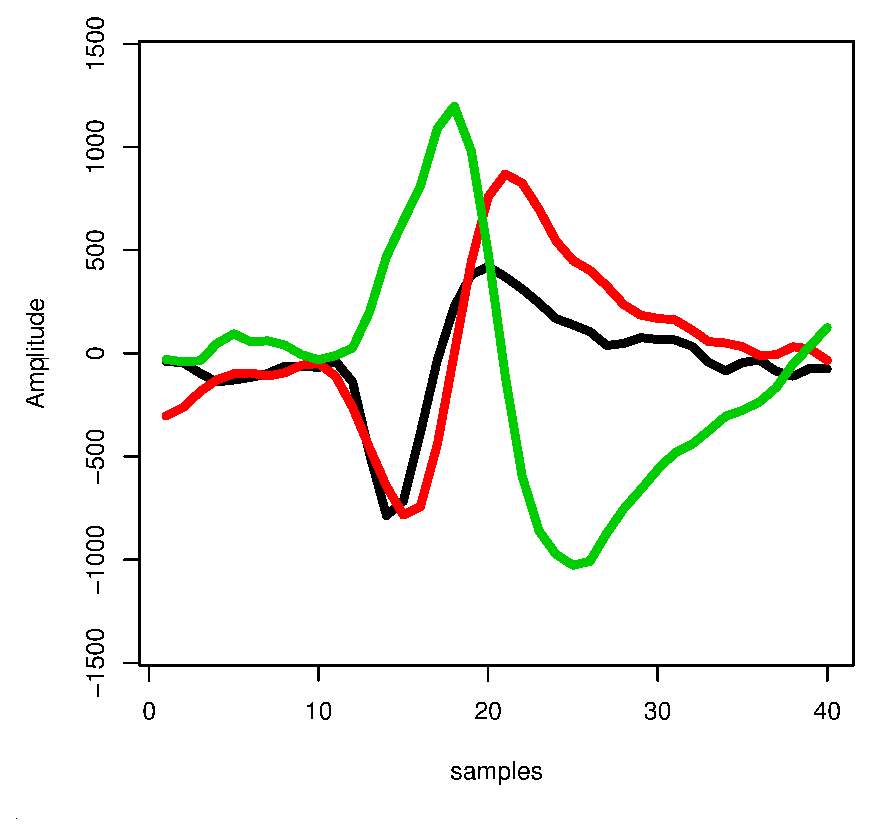
\includegraphics[width=15cm,keepaspectratio]{./fig/simu_2/template.eps}
	\caption{simulation 2: $B$=$l$>$l$N%F%s%W%l!<%HGH7A(B}
	\label{fig:simu_2_temps}
	\end{center}
\end{figure}

$B3F%9%Q%$%/GH7A$O!"<!$N(BEV$B%U%!%$%k$NCf$+$i!"GH7A$rFI$_9~$s$@$b$N$G$"$k!#(B
\begin{itemize}
 \item $B9u(B:rkcy00ep050.001.ev
 \item $B@V(B:0318aep005.011.ev
 \item $BNP(B:05-9Cep031.011.ev
\end{itemize}

\clearpage


%\begin{tabular}{|c|c|c|c|c|c|}
%  &$B%F%s%W%l!<%H(B& $B%9%Q%$%/$N?t(B&$\delta$&$\lambda$&$BJ?6QH/2PN((B  \\
% $B%K%e!<%m%s#1(B&rkcy00ep050.001.ev&35&0.8&100&0.040  \\
% $B%K%e!<%m%s#2(B&0318aep005.011.ev&35&0.8&100&0.035   \\
% $B%K%e!<%m%s#3(B&05-9Cep031.011.ev&30&0.8&150&0.200    \\
%\end{tabular} 

%
%\begin{figure}[htbp]
% \begin{tabular}{cc} %
%  \begin{minipage}{0.5\hsize}
%   
%   \begin{center}
%    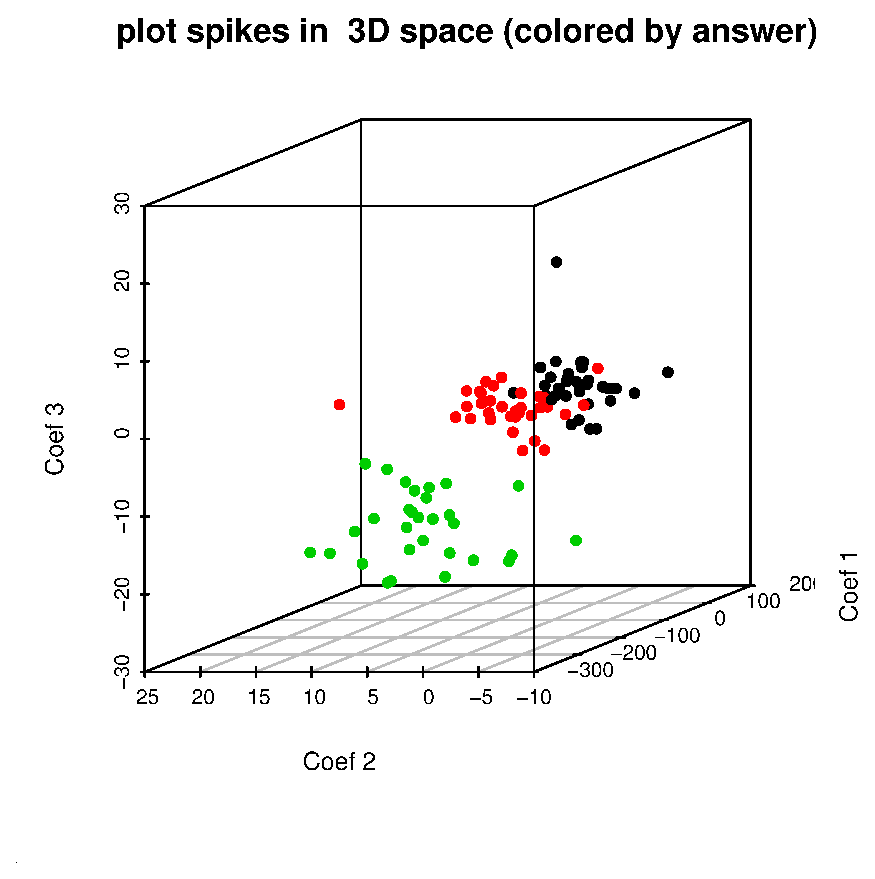
\includegraphics[width=10cm]{./fig/simu_2/SNR1wavelet_trueans.eps}
%    \caption{simu2: true labels}
%    \label{fig_simu_2_trueans}  
%   \end{center}
%
%  \end{minipage}
%  
%  %k-means
%  \begin{minipage}{0.5\hsize}
%    \begin{center}
%     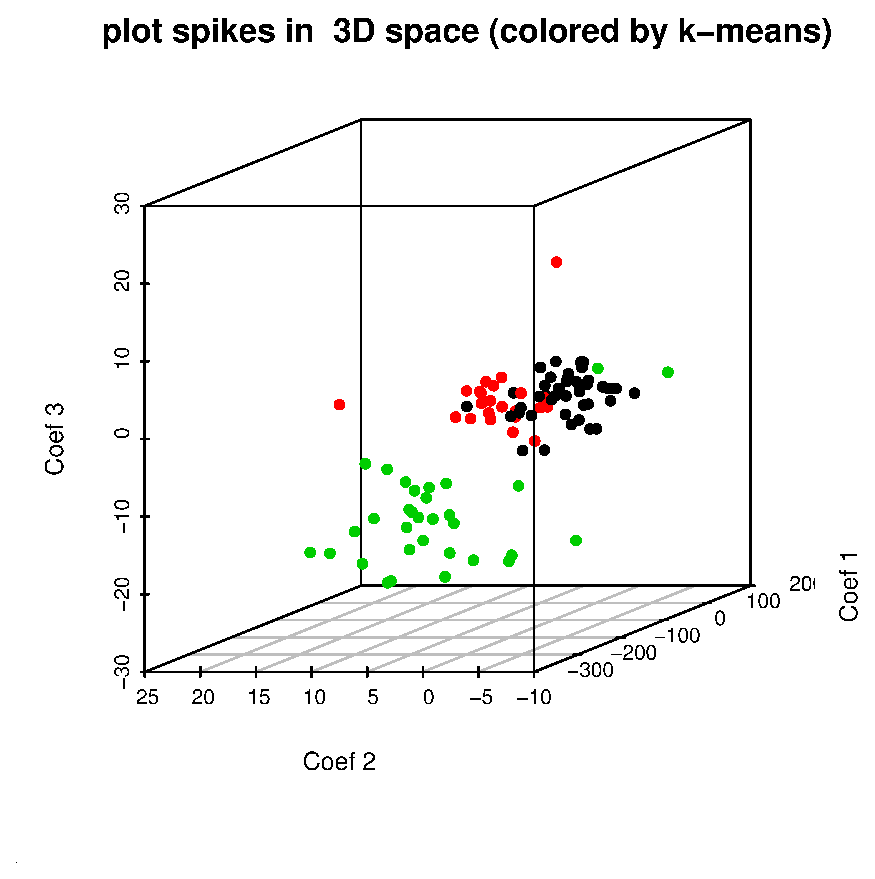
\includegraphics[width=10cm]{./fig/simu_2/SNR1wavelet_kmeans10.eps}
%     \caption{simu2: sorted labels}
%     \label{fig_simu_2_k-means} 
%  \end{center}
%
% \end{minipage}
%\end{tabular}
%
% %\caption{[A]$B@5$7$$%9%Q%$%/%i%Y%k$H(B[B]$B%=!<%F%#%s%08e$N%9%Q%$%/%i%Y%k(B}
%% \label{fig_simu_2}
%\end{figure}
%
%\begin{figure}
% \begin{center}
%    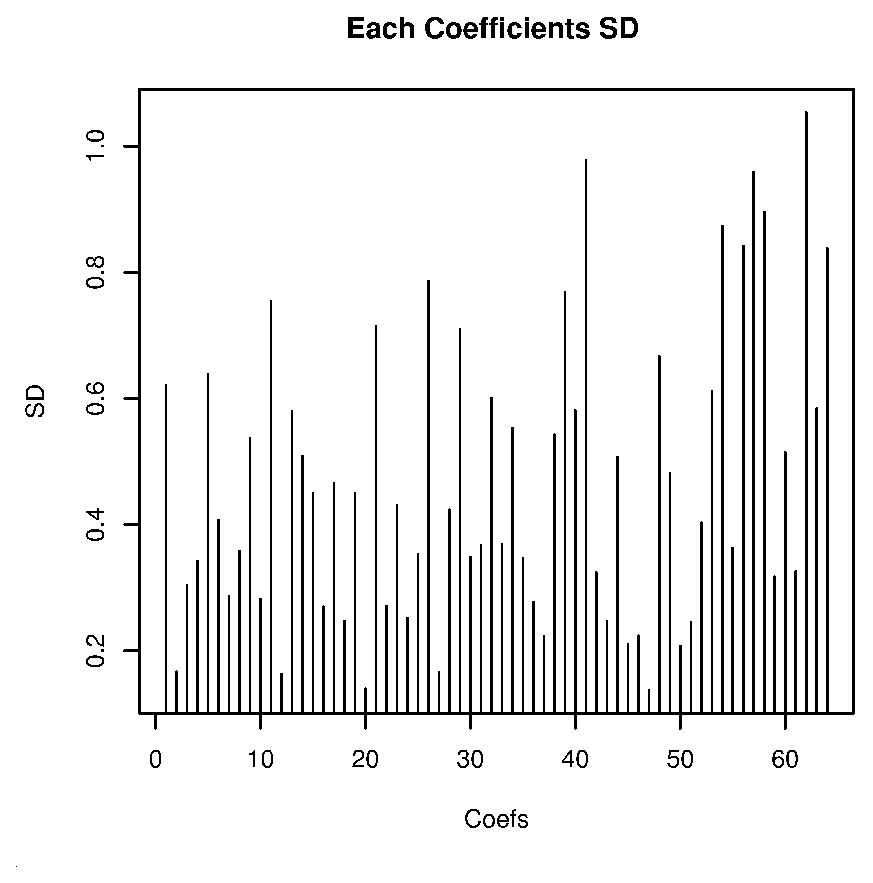
\includegraphics[width=10cm]{./fig/simu_2/SNR1Axes_Scores.eps}
% \end{center}
% \caption{simu 2: Each coeff's score}
% \label{fig_simu_1_score}
%\end{figure}
%
%\clearpage

%\begin{figure} [h] 
% \centering
% \subfigure[fig.a title]{
% \label{fig_a} 
% \resizebox{5cm}{6cm}{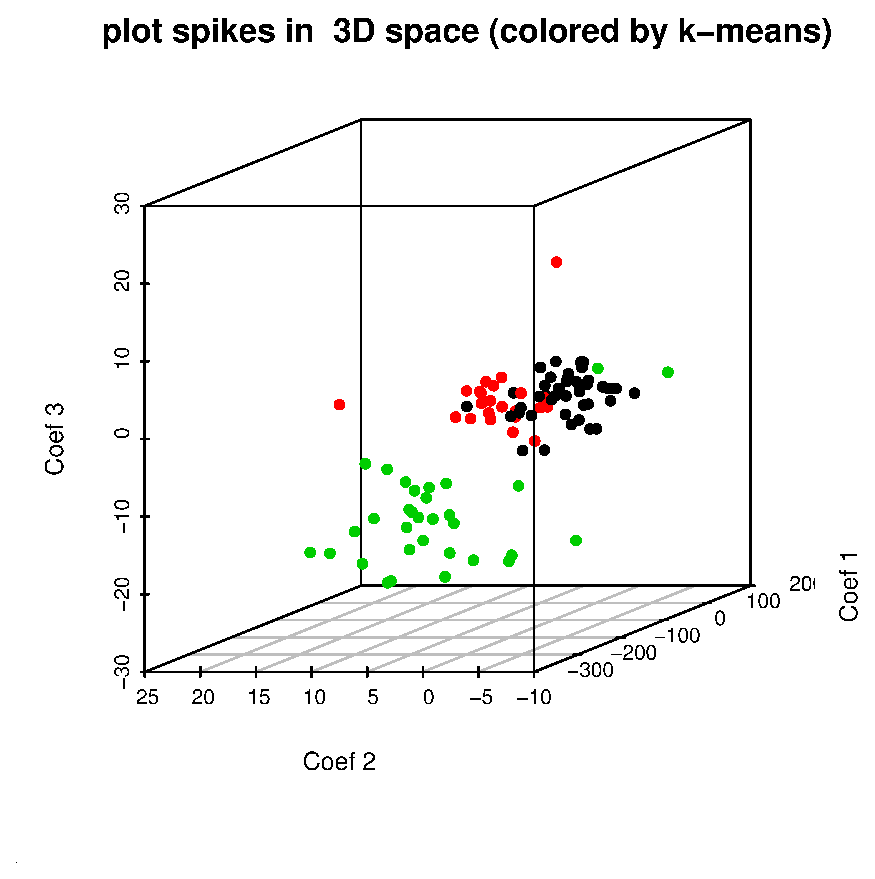
\includegraphics{./fig/simu_2/SNR1wavelet_kmeans10.eps}}}
% \subfigure[fig.b title]{
% \label{fig_b} 
% \scalebox{0.3}{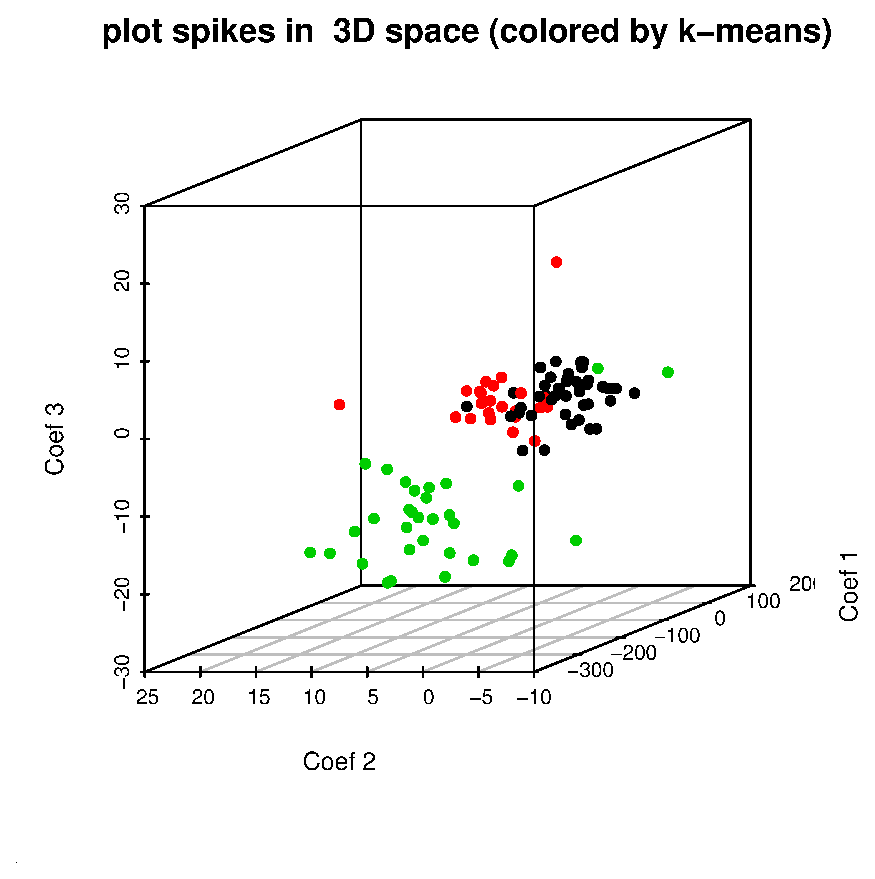
\includegraphics{./fig/simu_2/SNR1wavelet_kmeans10.eps}}}
% \subfigure[fig.c title]{
% \label{fig_c} 
% \resizebox{5cm}{1.4cm}{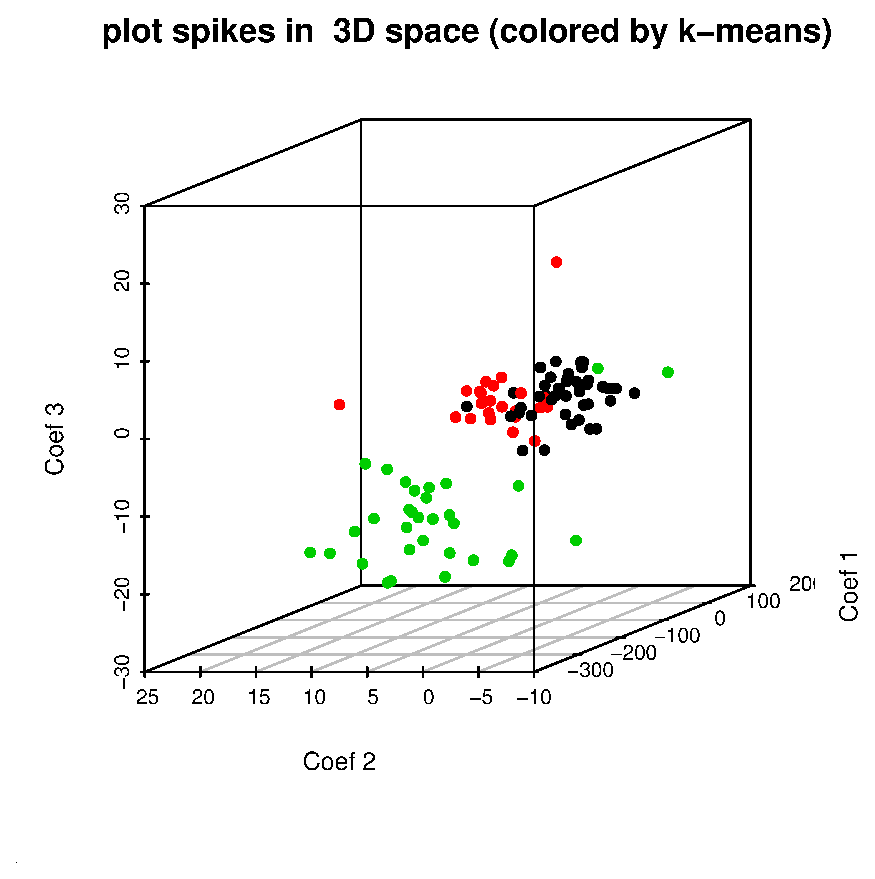
\includegraphics{./fig/simu_2/SNR1wavelet_kmeans10.eps}}}
% \caption{hoge1}
% \label{fig_total}
%\end{figure}

$B%7%_%e%l!<%7%g%s(B2

\begin{figure} [h] 
 \centering
 %true
 \subfigure[$B@52r(B]{
 \label{fig_a} 
 \resizebox{8cm}{8cm}{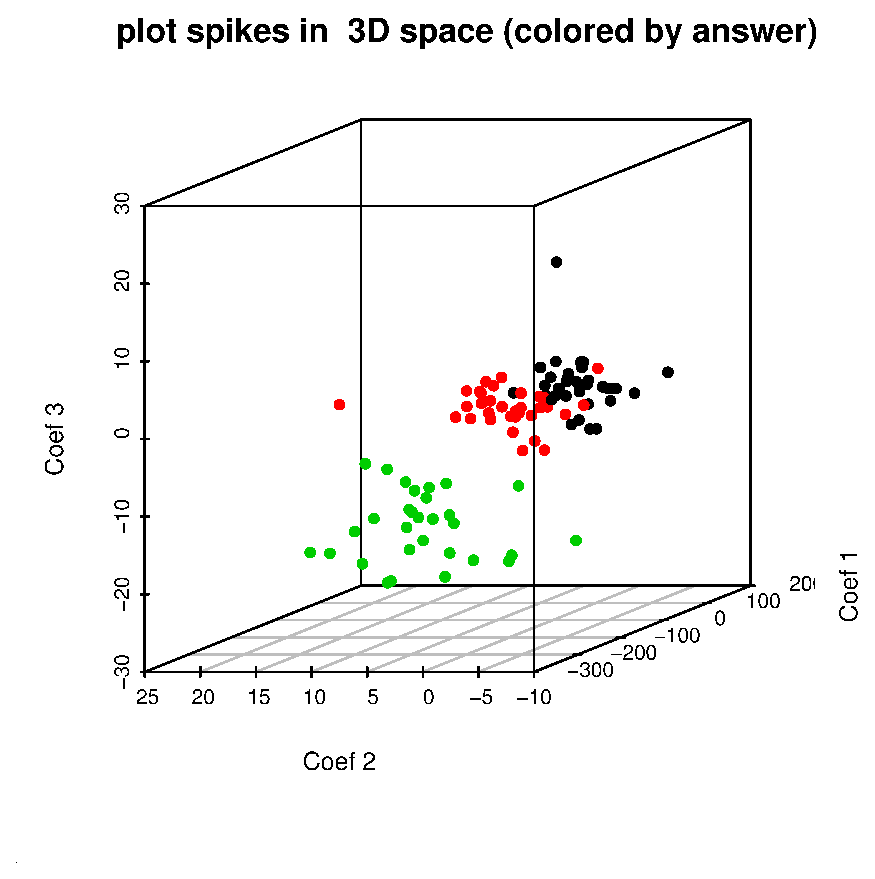
\includegraphics{./fig/simu_2/SNR1wavelet_trueans.eps}}}
 %k-means
 \subfigure[$B%=!<%F%#%s%08e(B]{
 \label{fig_b} 
 %\scalebox{0.3}{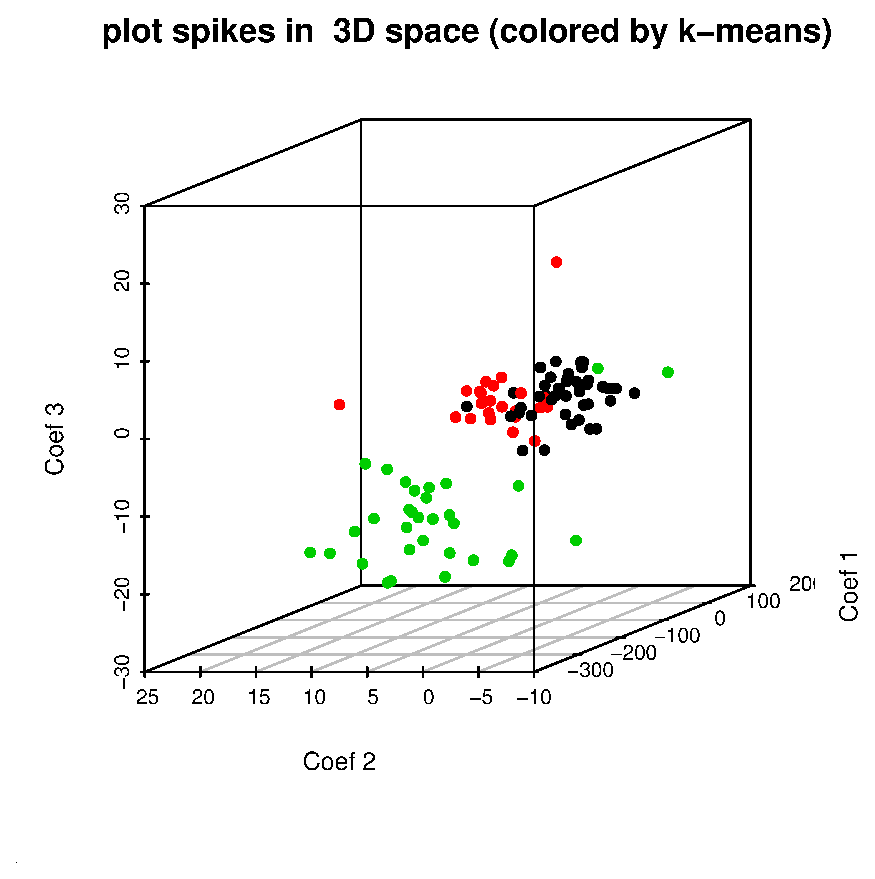
\includegraphics{./fig/simu_2/SNR1wavelet_kmeans10.eps}}}
 \resizebox{8cm}{8cm}{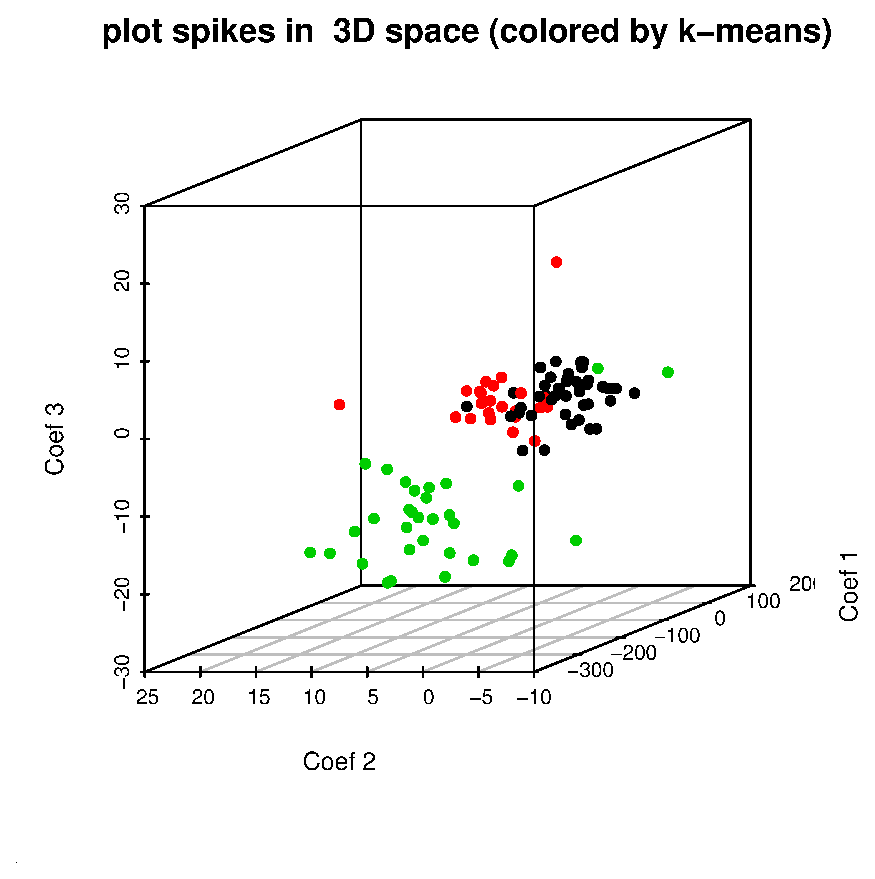
\includegraphics{./fig/simu_2/SNR1wavelet_kmeans10.eps}}}
\caption{simulation 2: $B%&%'!<%V%l%C%HJQ49$5$l$?%9%Q%$%/Ns(B}
%%wavelet sd
%\subfigure[fig.c title]{
% \label{fig_c}
% \resizebox{10cm}{10cm}{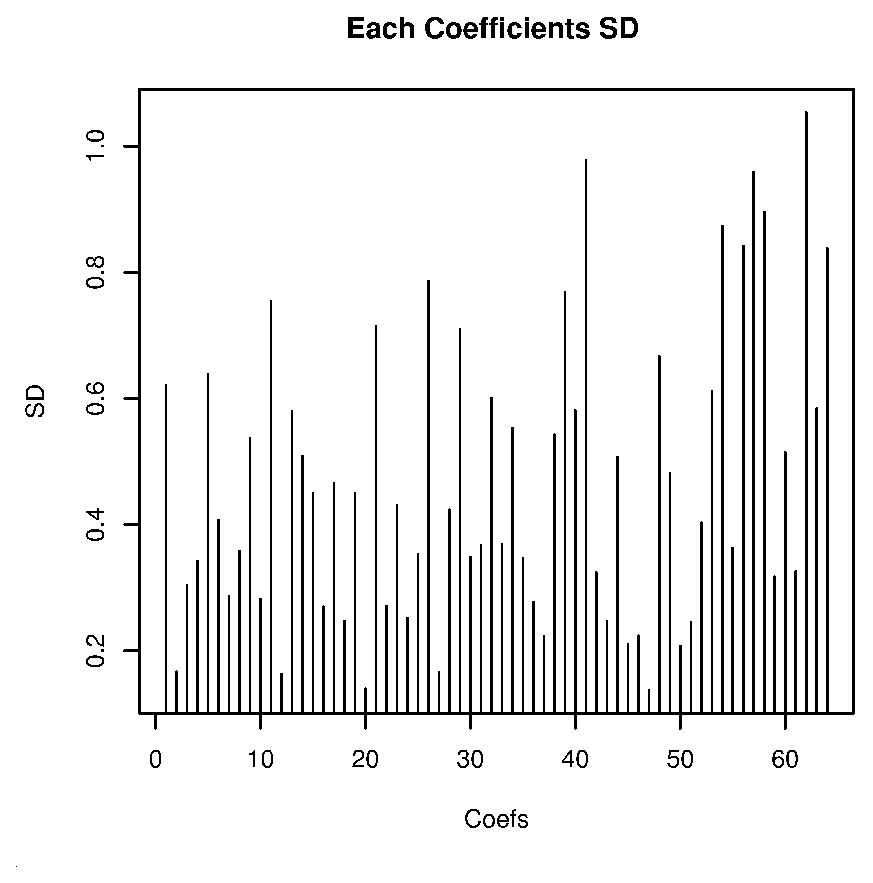
\includegraphics{./fig/simu_2/SNR1Axes_Scores.eps}}}
% \caption{$B4pDl4X?t(B$\phi_{1}\sim\phi_{64}$$B$NF@E@(B}
 \label{fig:simu_2}
\end{figure}
\begin{figure}[h]
 \begin{center}
    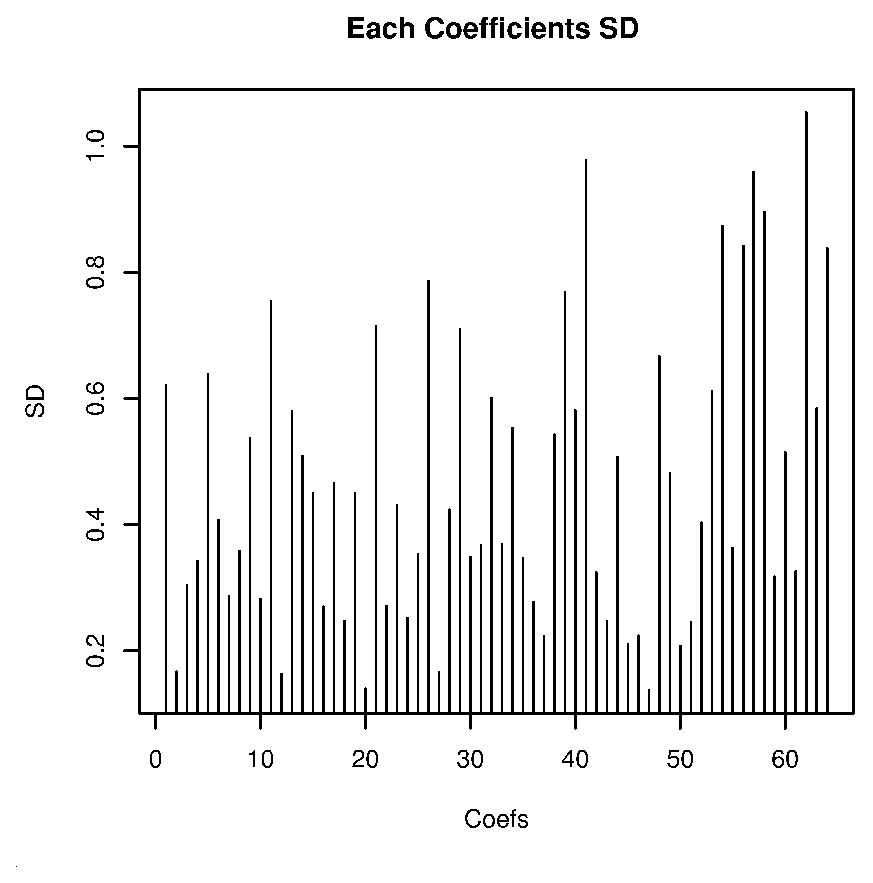
\includegraphics[width=7cm,height=7cm]{./fig/simu_2/SNR1Axes_Scores.eps}
 \end{center}
 \caption{simulation 2: $B4pDl4X?t(B$\phi_{1}\sim\phi_{64}$$B$NF@E@(B}
 \label{fig:simu_1_score}
\end{figure}

%\clearpage

\clearpage